\documentclass[handout, 10pt]{beamer}

%\usepackage[backend=bibtex,firstinits=true,style=verbose-inote,citestyle=authortitle]{biblatex}
\usepackage{bm}
\usepackage{graphicx}
\usepackage{subcaption}
\usepackage{amsmath}
\usepackage{amsfonts}
\usepackage{makecell}
\usepackage{filecontents}
\usepackage{biblatex}
% \newcommand{\expect}[2][]{
\ifthenelse{\equal{#1}{}}{
\mathbb{E}\left[#2\right]
}{
\underset{#1}{\mathbb{E}}\left[#2\right]
}}

\newcommand{\cov}[2][]{
\ifthenelse{\equal{#1}{}}{
\text{Cov}\left[#2\right]
}{
\underset{#1}{\text{Cov}}\left[#2\right]
}}


\newcommand{\var}[2][]{
\ifthenelse{\equal{#1}{}}{
\text{Var}[#2]
}{
\underset{#1}{\text{Var}}[#2]
}}

\newcommand{\loss}[2][]{
\ifthenelse{\equal{#1}{}}{
\mathcal{L}(#2)
}{
\mathcal{L}_{#1}(#2)
}}

\newcommand{\kl}[2]{
\text{D}_\text{KL}[#1 \parallel #2]
}

\newcommand{\R}{\mathbb{R}}
%\newcommand{\Prob}{\mathbb{P}}

\newcommand{\1}[1]{\mathds{1}\{#1\}}


%\usecolortheme{dolphin}
\setbeamertemplate{navigation symbols}{}
\setbeamertemplate{section in toc}{\inserttocsectionnumber.~\inserttocsection}

\newcommand{\expect}[2][]{
\ifthenelse{\equal{#1}{}}{
\mathbb{E}\left[#2\right]
}{
\underset{#1}{\mathbb{E}}\left[#2\right]
}}

\newcommand{\var}[2][]{
\ifthenelse{\equal{#1}{}}{
\text{Var}\left[#2\right]
}{
\underset{#1}{\text{Var}}\left[#2\right]
}}

\begin{filecontents*}{references.bib}
@inproceedings{
HyperNetsWeightInit,
title={Principled Weight Initialization for Hypernetworks},
author={Oscar Chang and Lampros Flokas and Hod Lipson},
booktitle={International Conference on Learning Representations},
year={2020},
url={https://openreview.net/forum?id=H1lma24tPB}
}
\end{filecontents*}

\addbibresource{references.bib}


\title{Principled Weight Initialization for Hypernetworks \footnote{\citepaper{HyperNetsWeightInit}}}
%\subtitle{}
%\author{Ivan Skorokhodov}
%\date{}
%\logo{
\includegraphics[height=1cm]{images/ipavlov-logo.png}}

\newcommand{\citepaper}[1]{\citetitle{#1} by \citeauthor{#1}}

%\graphicspath{{./images}}

%\usetheme{lucid}
\begin{document}

\begin{frame}
    \titlepage
\end{frame}

\begin{frame}{Overview}
\begin{itemize}
    \item\pause \textit{Hypernetwork} is a model that produces weights for another model (\textit{target model})
    \item\pause Hypernetworks are used in a lot of applications: mutli-task learning, continual learning, weights compression, etc. 
    \item\pause People use traditional initialization strategies (Xavier, He, etc) for hypernetworks
    \item\pause But these traditional initializations of a hypernetwork lead to a bad initialization of a target model
    \item\pause Authors fixed initialization for a hypernetwork to make the training more stable
\end{itemize}
\end{frame}

\begin{frame}{What is a hypernetwork?}
\begin{itemize}
    \item\pause Imagine we have a target model $f_\theta(x)$ which solves the task of interest
    \item\pause A hypernetwork $H_\phi$ produces the parameters for each layer $l$ of $f_\theta$ given an embedding $e_l$: $\theta_l = H_\phi(e_l)$.
    \item\pause During training we optimze parameters $\phi$ instead of $\theta$ by backpropagating $\Delta \theta$ further to $\Delta\phi$.
    \item\pause People usually use very small hypernetworks (1 or 2 hidden layers) since our output is very large
    \item\pause For example, for a dense layer of input-output sizes $500 \times 500$, our output layer for $H_\phi$ is $250,000$ neurons.
\end{itemize}
\end{frame}

\begin{frame}{Notation}
\pause We will use the following notation:
\begin{itemize}
    \item\pause Einstein summation:
\[
\alpha_i \beta^i = \sum_{i=1}^n \alpha_i \beta^i
\]
    \item\pause Denote by $W[t]$ a weight matrix in $t$-th layer for the main model
    \item\pause Then transformation $y^i = W[t]_j^i x^j + b^i$ means $y^i = W^{(t)}_i x + b^i$, i.e. $t_i$ is the $i$-th neuron and $W^{(t)}_i$ is the $i$-th row in the $t$-th layer's matrix $W^{(t)}$.
    \item\pause $\partial_x f = \frac{\partial f}{\partial x}$
    \item\pause Hypernetwork $H_\phi$ produces $W_j^i$ by:
    \[
    W_j^i = H_{jk}^i h(e)^k + \beta_j^i,
    \]
    where $e$ is a layer's embedding, $h$ is the hypernetwork's body, $H_{j}^i, \beta^i_j$ are output weights and biases ($H$ is a 3-dimensional tensor). 
\end{itemize}

\end{frame}

\begin{frame}{Xavier fan-in init}
    \pause Suppose we have a transformation $y^i = W_j^i x^j + b^i$. Xavier init is based on the following assumptions:
    \begin{enumerate}
        \item\pause $\forall i,j: W_j^i, x^j, b^i$ are independent from each other.
        \item\pause $\forall i,j: \expect{W_j^i} = 0$
        \item\pause $\forall j: \expect{x^j} = 0$
        \item\pause $\forall i: \expect{b^i} = 0$.
    \end{enumerate}
    
    \pause If these assumptions hold, then $\expect{y^i} = 0$ and:
    \[
    \var{y^i} = d_j \var{W_j^i} \var{x^j}
    \]

    \begin{itemize}
        \item\pause The goal of a good initialization is to make $\var{y^i} = \var{x^j}$.
        \item\pause This gives us $\var{W_j^i} = \frac{1}{d_j}$
    \end{itemize}
\end{frame}

\begin{frame}{Fan-out init and Kaiming inits}
    \begin{itemize}
        \item\pause On the previous slide, we tried to have $\var{y^i} = \var{x^j}$ during a forward pass.
        \item\pause But what if we want a similar property for a backward pass?
        \item\pause Since backprop for a linear layer gives $\partial_x \mathcal{L} = \partial_y \mathcal{L} W$
        then the similar reasoning leads to $\var{W_j^i} = \frac{1}{d_i}$. This is a \textit{fan-out} init.
        \item\pause Since we want both $\var{W_j^i} = \frac{1}{d_j}$ and $\var{W_j^i} = \frac{1}{d_i}$, which is impossible, let's just take their harmonic mean and set $\var{W_j^i} = \frac{2}{d_i + d_j}$
        \item\pause Kaiming inits are very similar, but we consider transformations like $y^i = W_j^i \sigma(x^j) + b^i$ for different non-linearities $\sigma$ (ReLU, LeakyReLU, tanh, etc), obtaining different initialization schemes.
    \end{itemize}
\end{frame}

\begin{frame}{Modern (ad-hoc) techniques of initializing hypernetworks}
    \pause Currently, people use the following schemes to initialize their hypernetworks:
    \begin{itemize}
        \item M1: Xavier or Kaiming inits
        \item M2: Small random values
        \item M3: Kaiming init, but with scaling output layer by 0.1
        \item M4: Kaiming init, but with scaling hypernetwork embeddings.
    \end{itemize}
    
    \pause
    \textbf{A problem}: using these initialization schemes in a hypernetwork produces such weights $W[t]$ in a target network that have bad variances $\var{W^i_j}$, making training difficult and unstable.
\end{frame}

\begin{frame}{Hyperfan-in assumptions}
    \pause First, authors make the following assumptions:
    \begin{itemize}
        \item\pause (1-4) Xavier assumptions for all the layers in the hypernet $h(e)$
        \begin{itemize}
            \item\pause This would give us $\operatorname{Var}\left(h(e)^{k}\right)=\operatorname{Var}\left(e^{l}\right)$
        \end{itemize}
        \item\pause (5) ...everything is independent of each other in the output layer
        \item\pause (6-8) ...everything has zero mean in the output layer
    \end{itemize}
\end{frame}

\begin{frame}{Hyperfan-in init}
    \pause
    Now, we want a transformation $y^i = W_j^i x^j + b^i$ not to change variance:
    \begin{itemize}
        \item\pause i.e, we want $\var{y^i} = \var{x^j}$
        \item\pause Using derivations similar to Xavier's ones, we can obtain:
\begin{equation}
\operatorname{Var}\left[H_{j k}^{i}\right]=\frac{1}{2 \mathrm{d}_{j} \mathrm{d}_{k} \operatorname{Var}\left[e^{m}\right]}
\end{equation}
        \item\pause This is a hyperfan-in init for hypernetworks.
        \item\pause If we want to generate biases for a target model as well, we would need to derive init for the corresponding component as well (you check the paper)
        \item\pause If we want hyperfan-out, this can be done in a similar manner
    \end{itemize}
\end{frame}

\begin{frame}{HyperKaiming inits}
    \begin{itemize}
        \item\pause On the previous slide, we had Xavier inits. But what if we care about activation functions?
        \item\pause Authors give an derivation for ReLU:
    \end{itemize}
    \begin{figure}
        \centering
        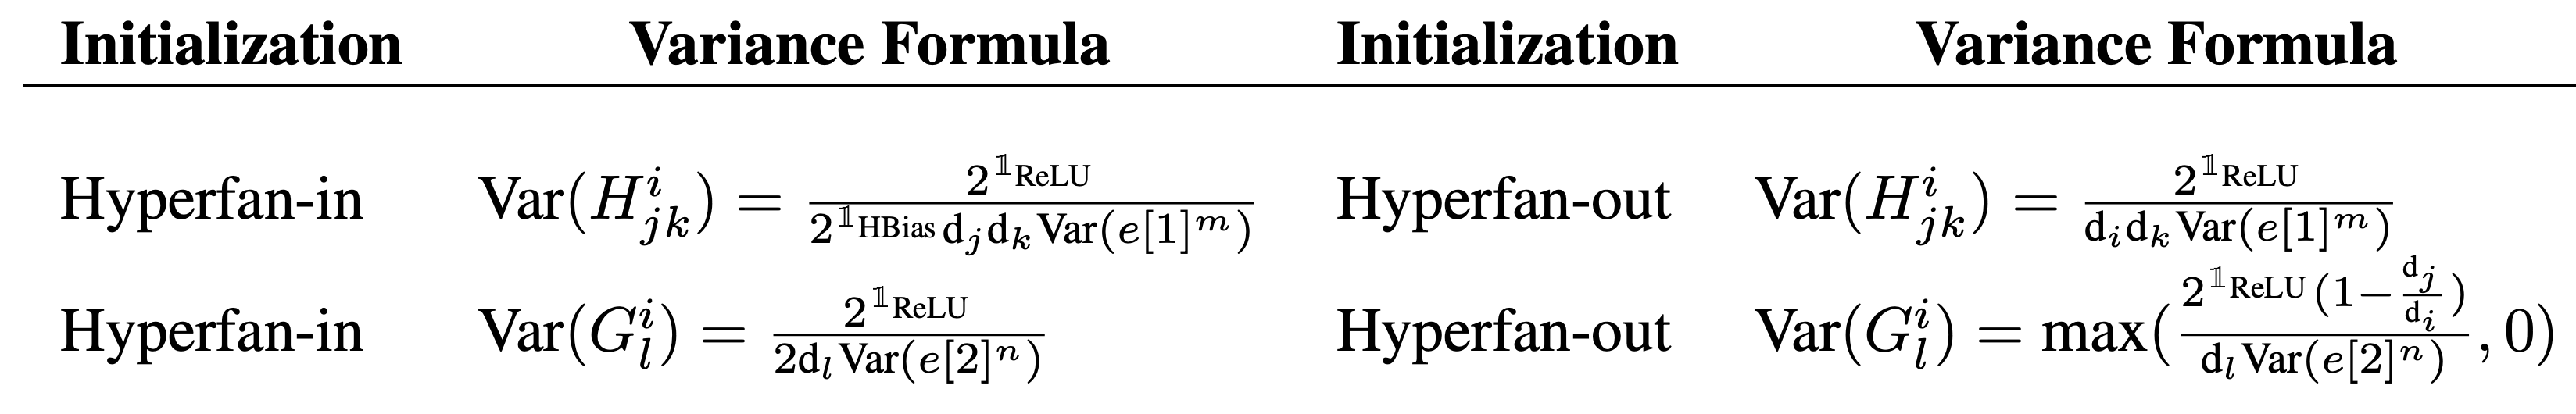
\includegraphics[width=\textwidth]{images/hyperkaiming.png}
    \end{figure}
    \begin{itemize}
        \item\pause For other activations, it should be derivable in a similar manner
    \end{itemize}
\end{frame}


\begin{frame}{Experiments: FeedForward Network on MNIST (1/2)}

\begin{figure}
    \centering
    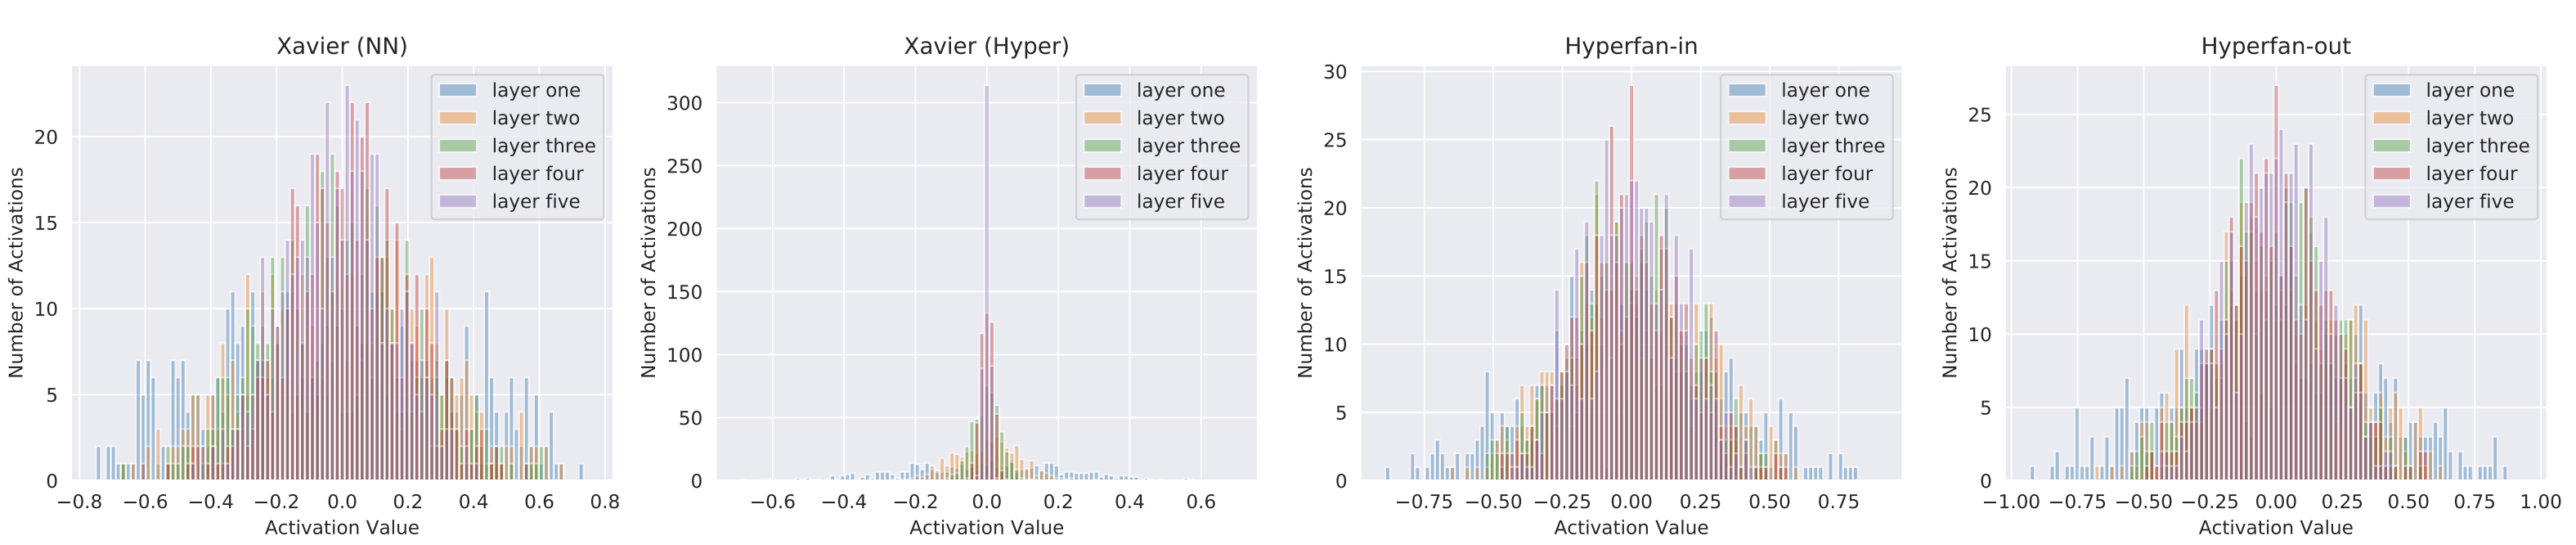
\includegraphics[width=\textwidth]{images/mnist-activations-before-training.png}
    \caption{MNIST mean activations before training}
\end{figure}

\begin{figure}
    \centering
    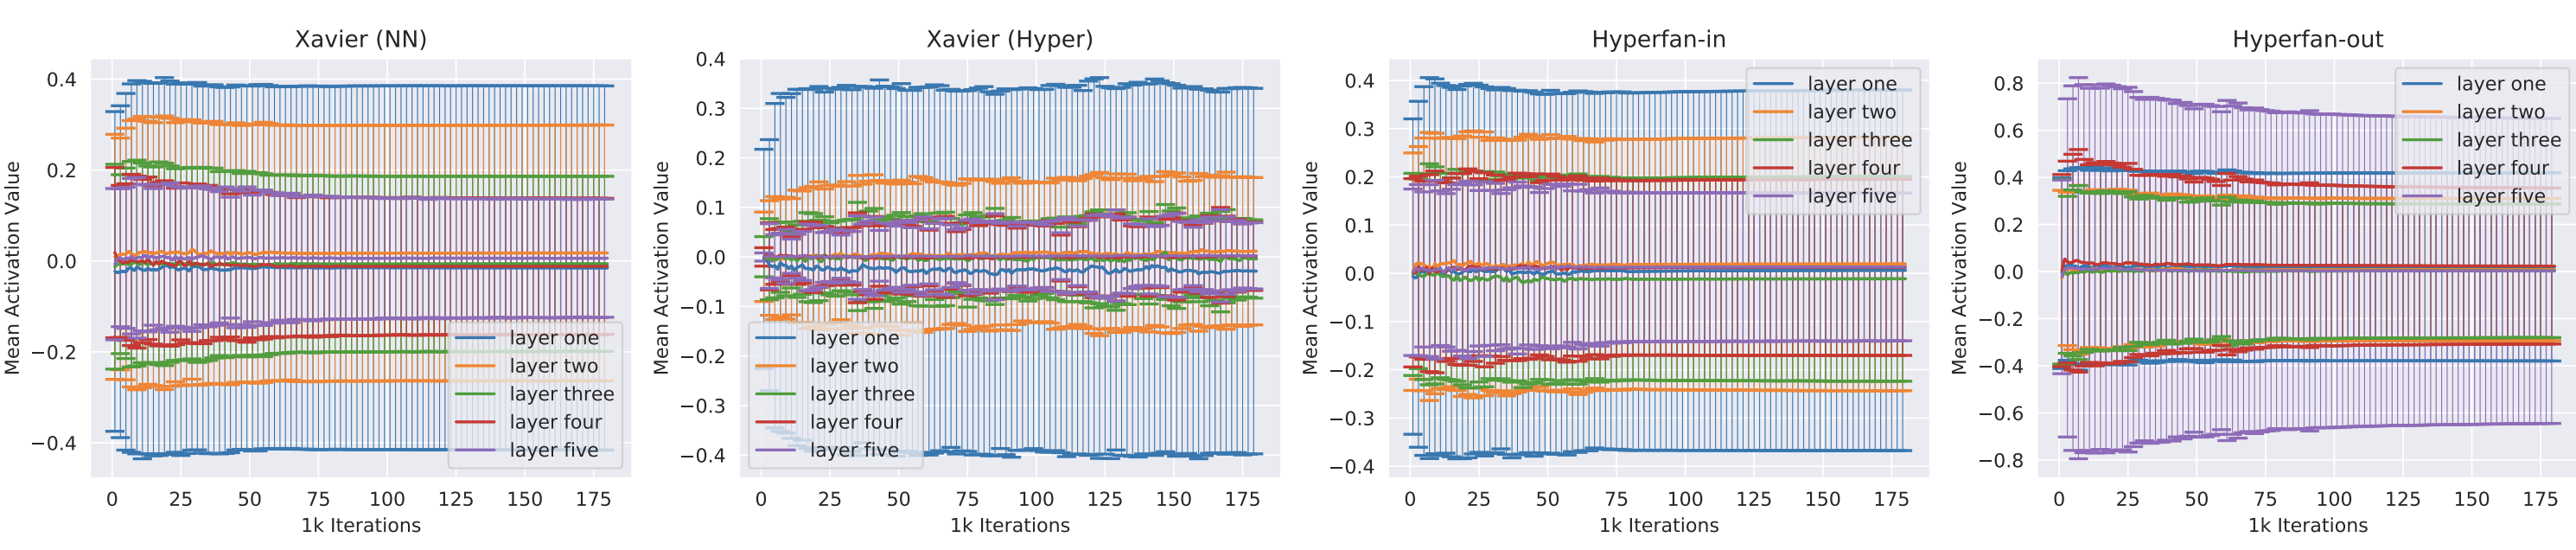
\includegraphics[width=\textwidth]{images/mnist-activations-evolution.png}
    \caption{MNIST activations evolution}
\end{figure}

\end{frame}

\begin{frame}{Experiments: FeedForward Network on MNIST (2/2)}
\begin{figure}
    \centering
    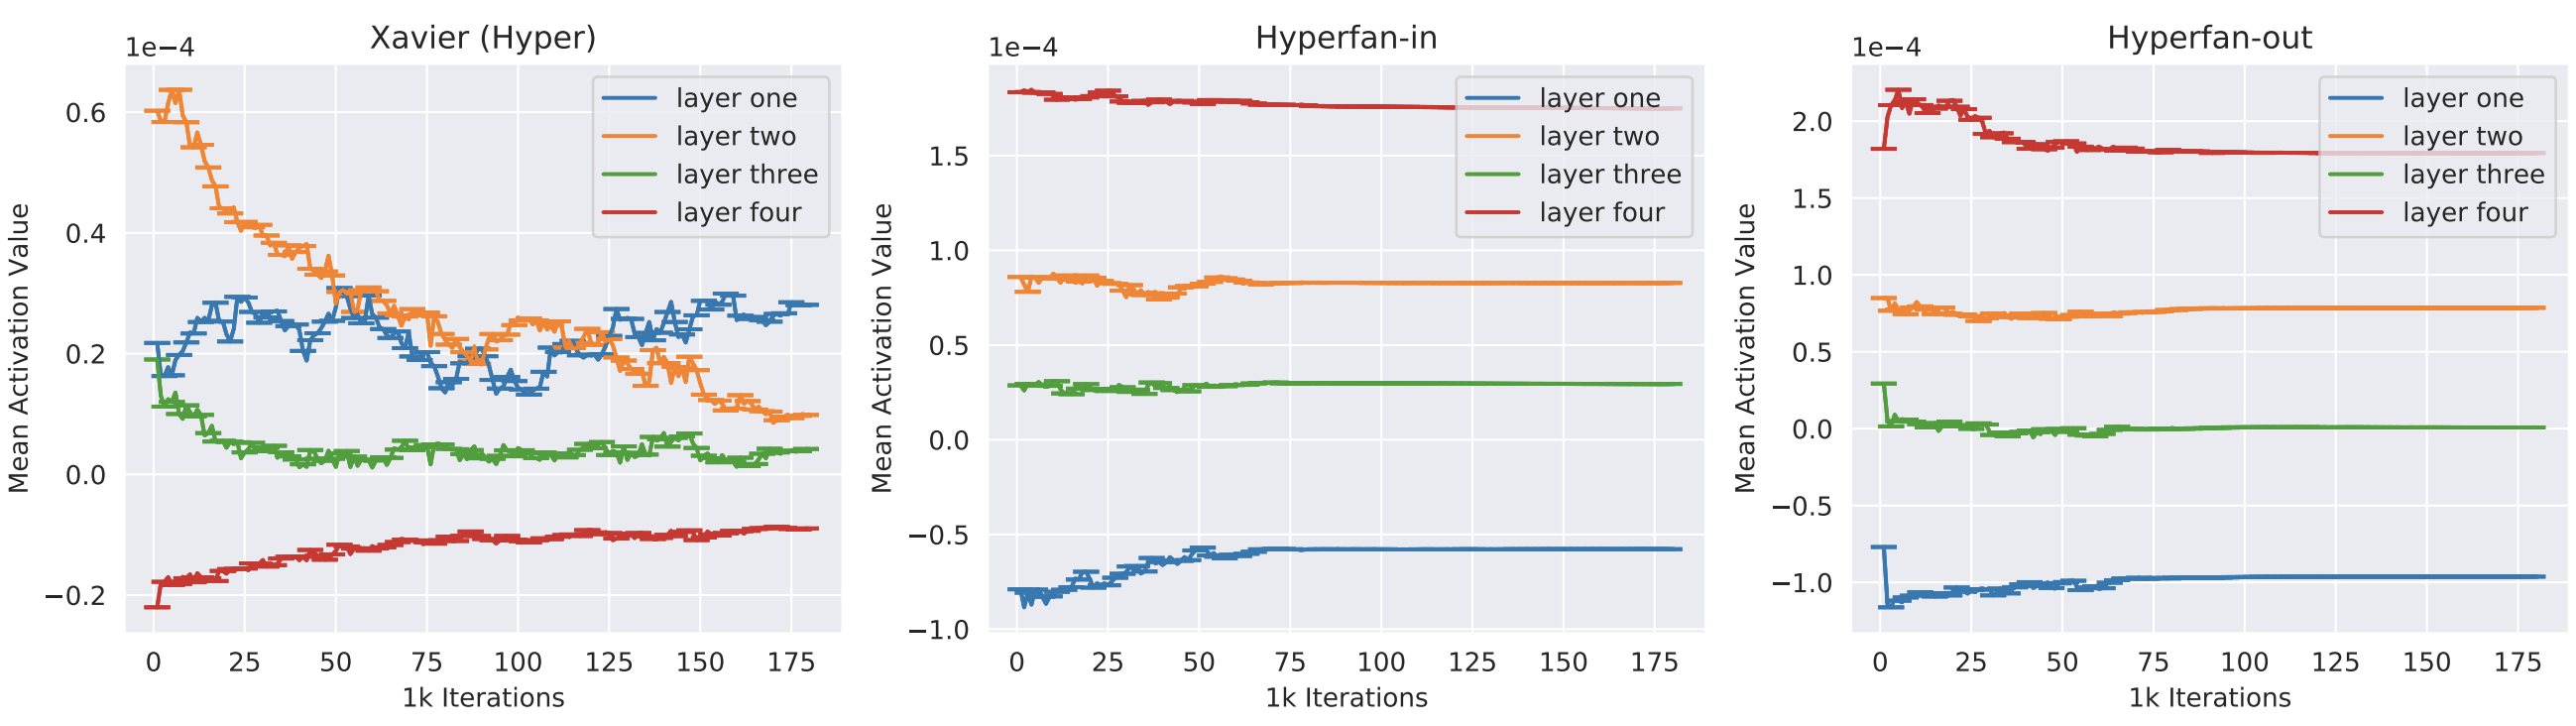
\includegraphics[width=\textwidth]{images/mnist-hypernet-mean-output.png}
    \caption{MNIST mean output value of $H_\phi(e)$}
\end{figure}

\begin{figure}
    \centering
    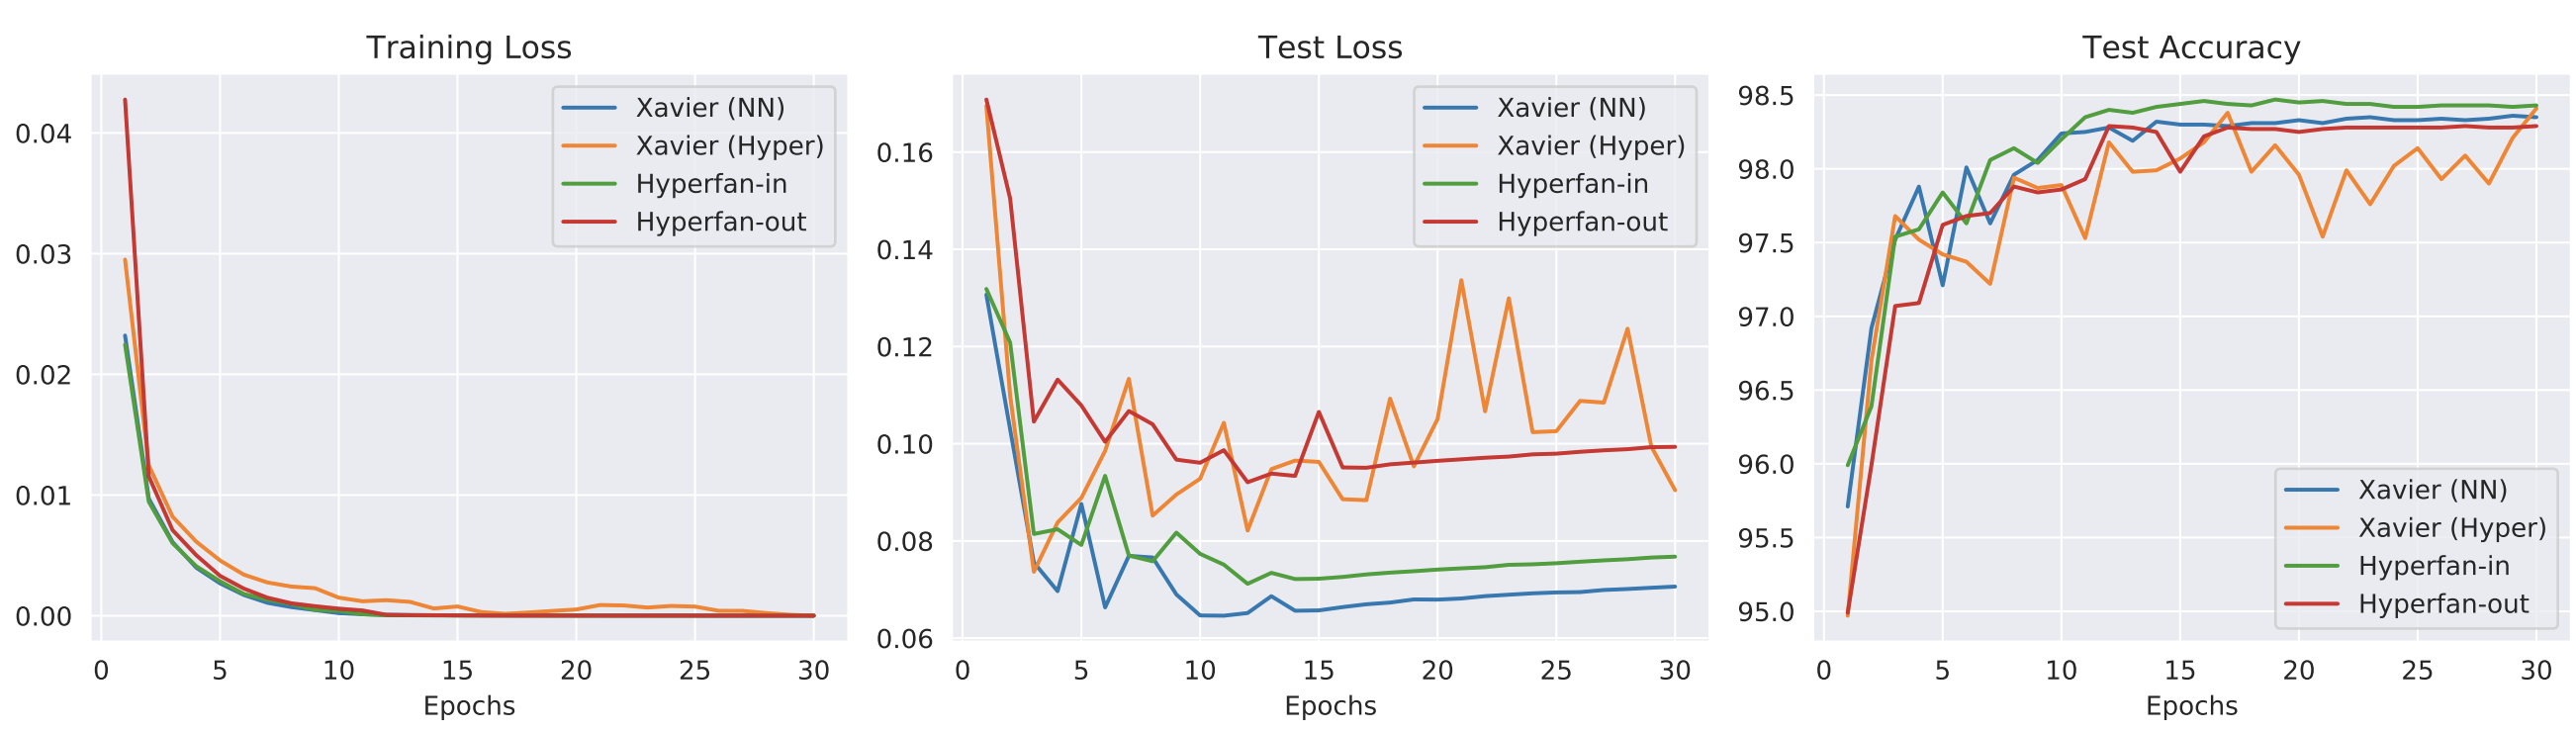
\includegraphics[width=\textwidth]{images/mnist-scores.png}
    \caption{MNIST train/test scores}
\end{figure}
\end{frame}


\begin{frame}{A bunch of final thoughts}
    \begin{itemize}
        \item Proper initialization is very important.
        \item The paper rises an important question of initialization for new architectures
        \item It is possible to derive Hyperkaiming inits for other non-linearities
        \item Authors' results on ImageNet for a bayesian NN looks suspicious ($\sim$17\% Top-5 accuracy for MobileNet after 25 epochs) 
    \end{itemize}
\end{frame}


\end{document}
